% Vorbereitung: Vorbereitungsaufgaben bearbeiten
% Versuchsaufbau: Verwendete Apparatur, Beschreibung Funktionsweise/Nutzen mit Skizze/Foto
\section{Durchführung}
\label{sec:durchführung}

Zur Versuchsdurchführung wurde der Aufabu aus \autoref{fig:aufbau1} verwendet.
\begin{figure}[H]
	\centering
	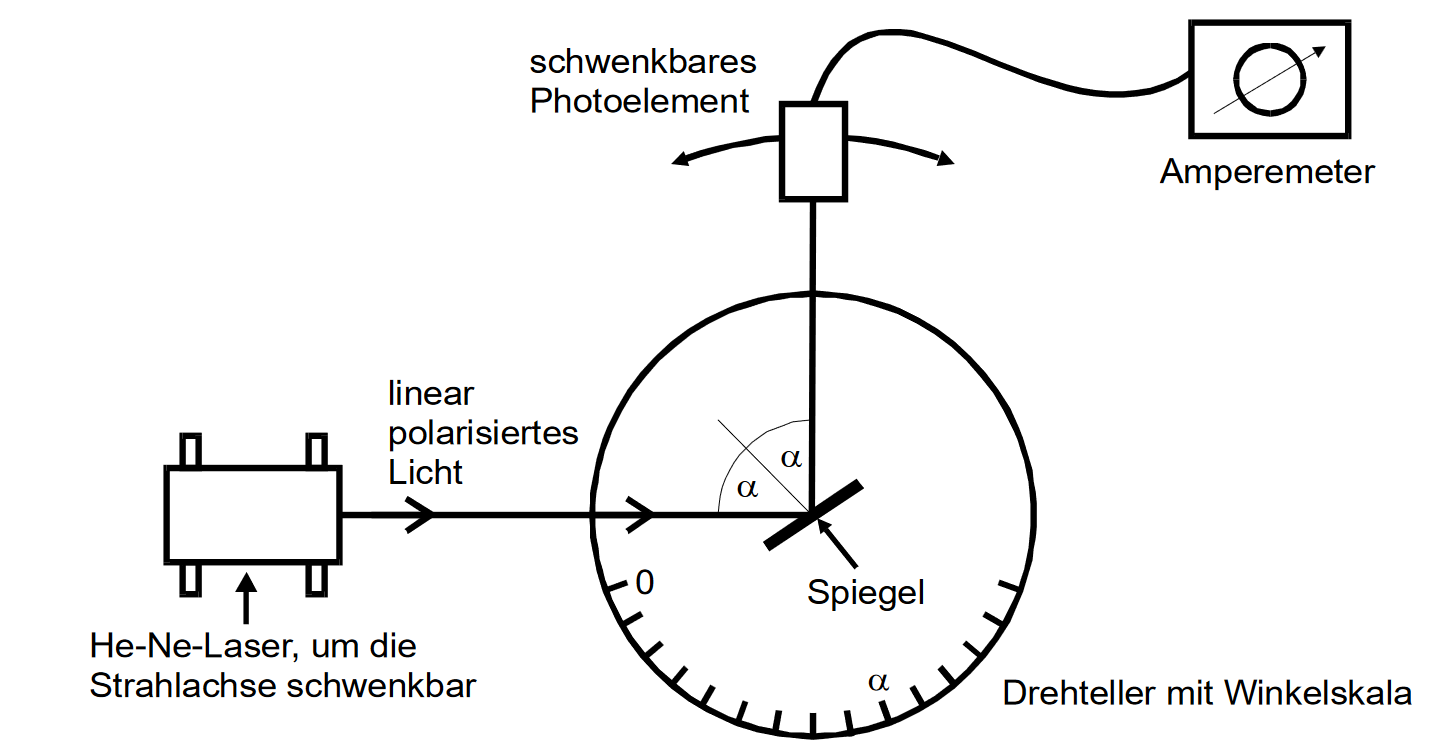
\includegraphics[width=0.6\linewidth]{content/grafik/aufbau1.png}
	\caption{Schematische Darstellung der verwendeten Messapperatur. \cite{fresnel}}
	\label{fig:aufbau1}
\end{figure}
Der lasertstrah des He-Ne-Lasers wird mithilfe des Polarisationsfilter polarisiert. Mit Hilfe des Goniometers lässt sich 
der Spiegel einstellen. Gemmessen wird mit einem schwenkbaren Photoelement.

In der \autoref{fig:aufbau2} ist das Goniometer mit aufgesetztem Probenhalter dargestellt.
\begin{figure}[H]
	\centering
	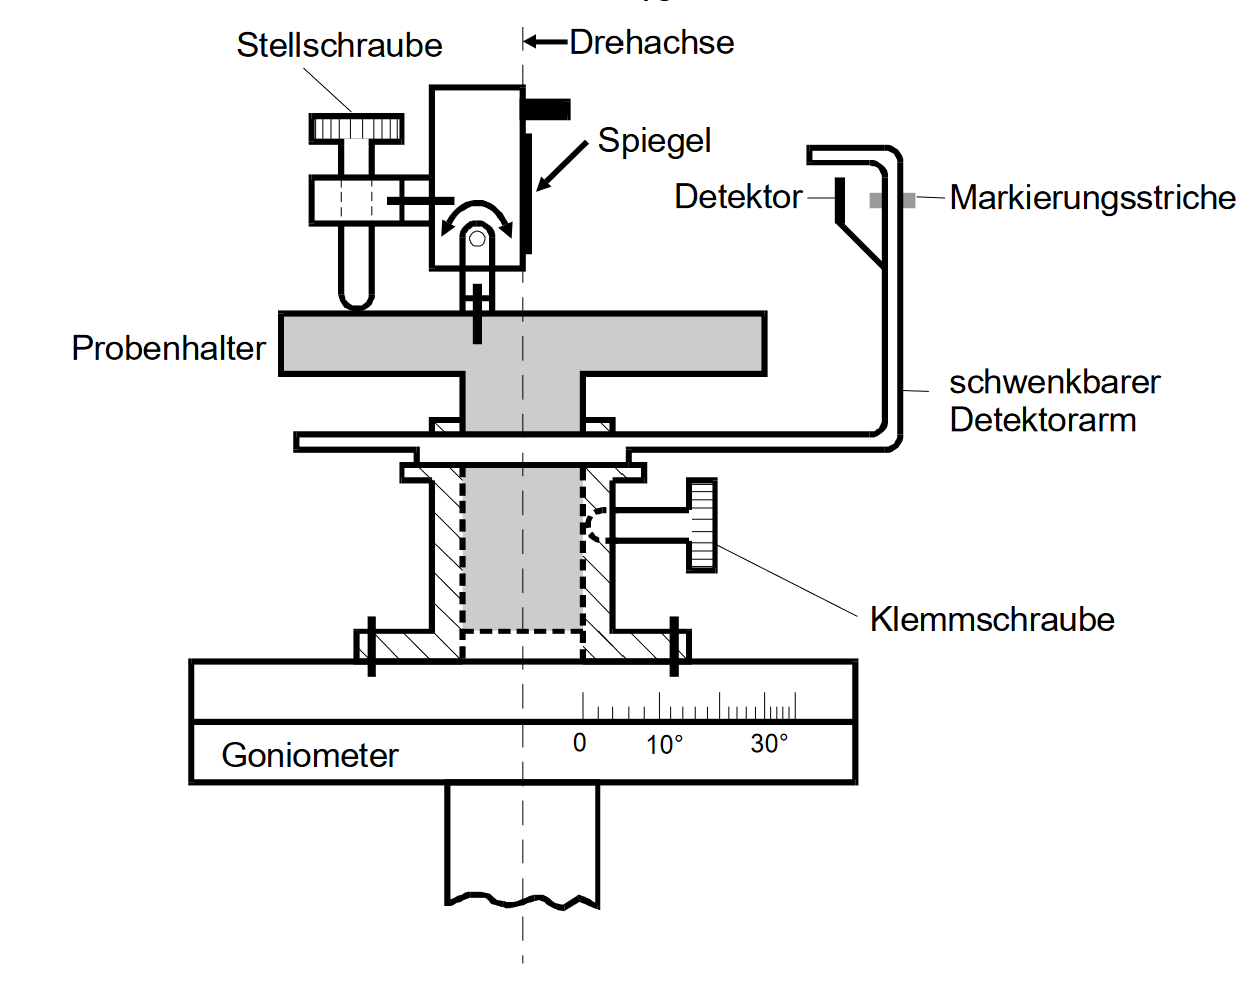
\includegraphics[width=0.6\linewidth]{content/grafik/aufbau2.png}
	\caption{Schematische Darstellung des Goniometers mit aufgesetztem Probenhalter. \cite{fresnel}}
	\label{fig:aufbau2}
\end{figure}
Der Spiegel ist mit einer Stellschraube befsetigt. Unterhalb des Probehalters ist die Haltung des Detektors befestigt

Bevor die Messung beginnt, werden der Dunkelstrom und den Photostrom des diskreten Lasers aufgenommen.
Daraufhin muss die Apperatur zunächst justiert werden. Der Probehalter wird aus den Strahlengang entfernt und der Detektor wird 
so eingestellt, dass der Laserstrahl direkt auf diesen trifft. Es wird der Polarisationsfilter
in den Strahlengang des Lasers eingebaut. Als erstes wird die Messung für s-polarisiertes Licht durchgeführt, dementsprechend 
wird der Winkel des Polarisationsfilters auf 0 gestellt. Der Drehteller mit der Winkelskala wird auf $\ang{0}$ eingestellt.
Die Skala des Drehtellers wird variiert. Die Messung startet bei $\ang{6}$, in $\ang{2}$-Schritten wird der Winkel größer, dabei
werden die Messwerte für die Stromstärke der Intensität aufgenommen. Der Vorgang endet bei $\ang{86}$. Analog verläuft 
der Mess-Vorgang für den Polarisationswinkel $\frac{\pi}{2}$.
